\begin{figure}[t]
\centering
% Vector drawing generated by tools/figures/build.py; rerun it after changing the figure.
\ifbilingual
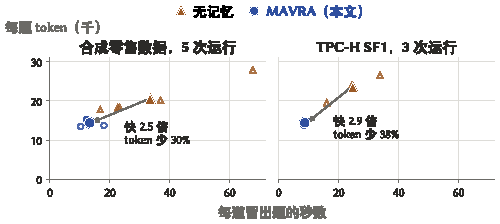
\includegraphics[width=\linewidth]{figures/consumer-cost-zh}
\else
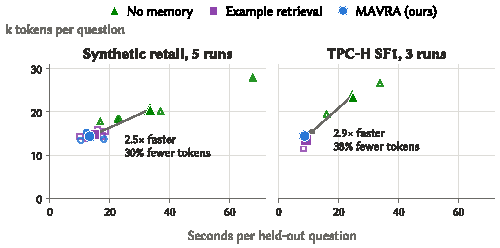
\includegraphics[width=\linewidth]{figures/consumer-cost}
\fi
\caption{\bt{What a consumer pays per held-out question on unchanged data: agent-session time and tokens per question. Small hollow markers are single runs, large markers pool all questions of a method; the arrow runs from exploring alone to \system.}{数据不变时使用者每道留出题的代价：每题的智能体会话时间与 token。小的空心标记为单次运行，大标记合并一种方法的全部题目；箭头从独自探索指向 \system。}}
\label{fig:consumer}
\Description{Two scatter plots of seconds against thousands of tokens per held-out question for no memory, example retrieval, and MAVRA. Synthetic retail dataset, five runs: exploring alone takes 33.4 seconds and 20.5 thousand tokens per question, MAVRA 13.2 seconds and 14.4 thousand, example retrieval 14.9 seconds and 14.8 thousand; the arrow is labelled 2.5 times faster with 30 percent fewer tokens. TPC-H SF1, three runs: exploring alone 24.7 seconds and 23.4 thousand tokens, MAVRA 8.7 seconds and 14.4 thousand, example retrieval 9.0 seconds and 13.5 thousand; the arrow is labelled 2.9 times faster with 38 percent fewer tokens.}
\end{figure}
